\documentclass[11pt]{article}
\usepackage{color}
\usepackage{authblk}%allows footnote format for authors
\usepackage[letterpaper, margin=1in]{geometry} %package that allows changes in margins and header/footers
\usepackage[sort]{natbib}
\usepackage{amsmath}
\usepackage{rotating}
\usepackage{adjustbox}
\usepackage[english]{babel}
\usepackage{colortbl}
\usepackage{booktabs}
\usepackage{tabularx}
\usepackage[x11names,dvipsnames,table]{xcolor}
\usepackage{lineno}
\linenumbers
\usepackage{array}
\newcolumntype{G}[1]{>{\raggedright\let\newline\\\arraybackslash\hspace{0pt}}m{#1}}
\newcolumntype{C}[1]{>{\centering\let\newline\\\arraybackslash\hspace{0pt}}m{#1}}
\bibliographystyle{NewPhyt.bst}
\renewcommand{\baselinestretch}{1.5}
\newcommand{\mbh}[1]{\textcolor{orange}{ \emph{\scriptsize  #1}} } %creating command for Matt's comments
\newcommand{\lwang}[1]{\textcolor{red}{ \emph{\scriptsize  #1}} } %creating command for Li's comments
\newcommand{\gmj}[1]{\textcolor{blue}{ \emph{\scriptsize  #1}} } %creating command for Garrett's comments

\title{Research Review: \\The Extent of Adaptive Wild Introgression in Crops}

\author[1]{Authors: Garrett M. Janzen}%author information
\author[1]{Li Wang}
\author[1,*]{Matthew B. Hufford}
\affil[1]{Department of Ecology, Evolution, and Organismal Biology, Iowa State University, Ames, Iowa, USA}
\affil[*]{Correspondence: email: mhufford@iastate.edu, telephone: 1-515-294-8511}
\date{}

\begin{document}

\maketitle

Number of Figures: 2, both in color

Number of Tables: 2

Word Count: 3,966

\clearpage

\section*{Summary}
The study of crop evolution has focused primarily on the process of initial domestication.
Post-domestication adaptation during the expansion of crops from their centers of origin has received considerably less attention.
Recent research has revealed that, in at least some instances, crops have received introgression from their wild relatives that has facilitated adaptation to novel conditions encountered during expansion.
Such adaptive introgression could bear importantly on the basic study of domestication, affecting estimates of several evolutionary processes of interest (\emph{e.g.}, the strength of the domestication bottleneck, the timing of domestication, the targets of selection during domestication).
Identification of haplotypes introgressed from the wild may also aid the identification of alleles that are beneficial under particular environmental conditions.
Here we review mounting evidence for substantial adaptive wild introgression in several crops and consider the implications of such gene flow to our understanding of crop histories.


\textbf{Key Words:} adaptation, domestication, gene flow, introgression, wild relatives

\section*{Introduction}

Plant domestication is often conceptualized as a geographically constrained process, with crops originating from a wild progenitor within defined centers followed by expansion to the modern-day range of cultivation \citep{Harlan1992}.
However, archaeological and genetic evidence are beginning to reveal that, in many cases, domestication has been temporally protracted and geographically diffuse \citep{Meyer2016, Wang2017, Fuller2014}.
An additional aspect of the emerging complexity of domestication is the occurrence of beneficial gene flow from locally adapted wild relatives to crops during their expansion following domestication.
It is this adaptive introgression that is the subject of this review.

Adaptive introgression has three components: hybridization between differentiated taxa, backcrossing to one of the parents, and selection on recombinant genotypes with progressively diminished linkage drag \citep{barton2001role}.
In domesticated species, adaptive introgression would consist of crop-wild hybrids backcrossing to a crop followed by increase in frequency of adaptive wild alleles in the crop and selection against undesirable wild background.
To date, the literature on crop-wild gene flow has largely focused on the risk of transgene introgression from domesticated crops into wild relatives (for a review, \citealt{stewart2003transgene}) and on modern plant breeding efforts to introgress desirable traits from wild relatives (for a review, \citealt{Dempewolf2017}).
The potential for adaptive introgression of wild alleles into domesticated crops over evolutionary timescales has received considerably less attention.
Recently developed methods have been applied to high-density marker data to detect genome-wide patterns of introgression, granting novel insight into the prevalence of adaptive introgression in crop histories.
Results from these studies suggest there is a need to expand our conception of domestication to encompass the broadening of the genetic base of crops that occurred through adaptive gene flow from newly encountered wild relatives during post-domestication expansion.

In this review, we: 1) briefly describe recent methods for detecting introgression, 2) present case studies suggesting wild-to-crop introgression has conferred local adaptation, 3) consider how introgression bears upon fundamental questions of domestication, and 4) describe key questions regarding crop adaptation through gene flow from wild relatives.


\section*{Introgression methods and their application}


The decreasing cost of genome-wide resequencing and availability of reduced-representation genotyping (\emph{e.g.}, GBS and RAD-Seq), combined with new analytical methods (\textbf{Table 1}), has facilitated comprehensive study of introgression across a broad spectrum of species.
The methods reviewed here do not include those estimating introgression\slash migration rate as a component of broader demographic history (\emph{e.g.}, Approximate Bayesian Computation (ABC; \citealt{beaumont2002}), diffusion approximations for demographic inference ($\delta a\delta i$; \citealt{gutenkunst2009}), isolation with migration models \citep{hey2004}, and methods utilizing the sequentially Markovian coalescent (\emph{e.g.}, PSMC; \citealt{li2011}). 
Rather, we focus on three categories of methods that explicitly identify introgressed genomic segments based on the extent of differentiation, patterns of nucleotide/haplotype sharing, and phylogenetic relationships.

First, introgressed segments are expected to show low differentiation from their source population.
The $F_{st}$ and $d_{XY}$ statistics and derivates of $d_{XY}$ including $G_{min}$ \citep{geneva2015} and $RND_{min}$ \citep{rosenzweig2016} gauge differentiation. 
The former two statistics are insensitive to rare migrants in a population and therefore lack power to detect very recent introgression, while the latter two overcome this limitation.
These statistics have been further developed by adding differentiation between both non-admixed ($A$) and admixed populations ($B$) and a source population ($C$) \citep{racimo2016}. 
For example, the $U_{A,B,C(w,x,y)}$ statistic summarizes the number of sites where an allele at frequency $y$ in the source population ($C$) has a frequency higher than $x$ in the admixed population ($B$) and lower than $w$ in the non-admixed population ($A$).
A similar statistic, $Q95_{A,B,C(w,y)}$, sets a hard cutoff at the $95^{th}$ percentile of allele frequency in the admixed population (B) \citep{racimo2016}.
Further modifications have allowed specification of more than one source population (see details in \citealt{racimo2016}).
Since differentiation-based methods can be calculated site-by-site, high-density, genome-wide data are not necessarily required.
However, accuracy of introgression estimates is improved with more comprehensive data.
Phased data are also not a prerequisite for differentiation-based methods.
 
Second, ancestry deconvolution (also known as local-ancestry inference and chromosome painting) assigns genomic regions to source populations based on patterns of allele or haplotype sharing \citep{schraiber2015}. 
One form of ancestry deconvolution utilizes a hidden Markov model to evaluate ancestry across admixed genomes through comparison to reference, non-admixed individuals (\emph{e.g.}, HAPMIX \citealt{Price2009}). 
Another clusters admixed populations with reference samples using a sliding-window approach (\emph{e.g.}, PCAdmix, \citealt{brisbin2012pcadmix} and LAMP, \citealt{sankararaman2008}).
A third version uses a Bayesian model \citep{pritchard2000} in which deviations from Hardy-Weinberg equilibrium are minimized through creation of genetic groups (\emph{e.g.}, fineSTRUCTURE, \citealt{Lawson2012}).
Ancestry deconvolution methods are better suited to high-density marker data given the intent to assign ancestry genome-wide.
Many such methods also require accurate phasing of haplotypes.

Phylogenetic relationships are applied to introgression detection using the ABBA-BABA statistic (also known as the D-statistic) and related metrics \citep{durand2011}.
These statistics make inferences regarding introgression based on genomic patterns of derived variants that are shared between populations or species.
While the D-statistic is best suited to detection of introgression at the genome level, elaborations of the D-statistic including $\hat{f_{d}}$ \citep{martin2015} and $D_{\textrm{FOIL}}$ tests \citep{pease2015} are capable of localizing introgression to specific chromosomal regions. 
The former is quite similar to the D-statistic but is based on allele frequencies, and the latter can identify donor and recipient lineages of introgression in a more complex, five-taxon phylogeny.
Like differentiation methods, phylogeny-based detection of introgression can be employed using low-density data.
However, because these methods require knowledge of whether an allele is ancestral or derived, data from a sufficiently diverged outgroup must be available.

Collectively, introgression detection methods have been applied to several systems, frequently identifying instances of adaptive introgression (see applications in \textbf{Table 1}).
For example, based on sequence divergence methods, introgression has been detected in \emph{Mimulus} (\emph{i.e.}, monkeyflower) species and appears to play a role in adaptation to pollinator preference and speciation \citep{Stankowski2015}.
Likewise, the HAPMIX ancestry deconvolution method was applied by \citet{jeong2014} to detect introgression from the Nepalese Sherpa to Tibetans at loci controlling high altitude adaptation.
Finally, the ABBA-BABA statistic has revealed introgression at wing coloration loci conferring M\"{u}llerian mimicry across butterfly species \citep{heliconius2012}.
Below we describe the nascent application of these methods to crop systems as well as implications for the study of domestication and adaptation.

\section*{Crop adaptation through introgression}

As range-wide genetic analyses of crops and their wild relatives have become feasible, evidence for substantial crop-wild introgression has been discovered in many important crops (\textbf{Table 2}).
Below we present a summary of findings from maize, barley, rice, and potato, four systems in which crop-wild gene flow appears to have played an adaptive role.
All four of these crops were domesticated in defined centers and have subsequently expanded to global distributions, a migration that brought them into contact with new populations of wild relatives that are distributed across broad environmental gradients (\textbf{Figure 1}).
For each case study we describe both what is known about a crop's domestication history and the prevalence of adaptive introgression during expansion.

\begin{figure}[h]
	\centering
	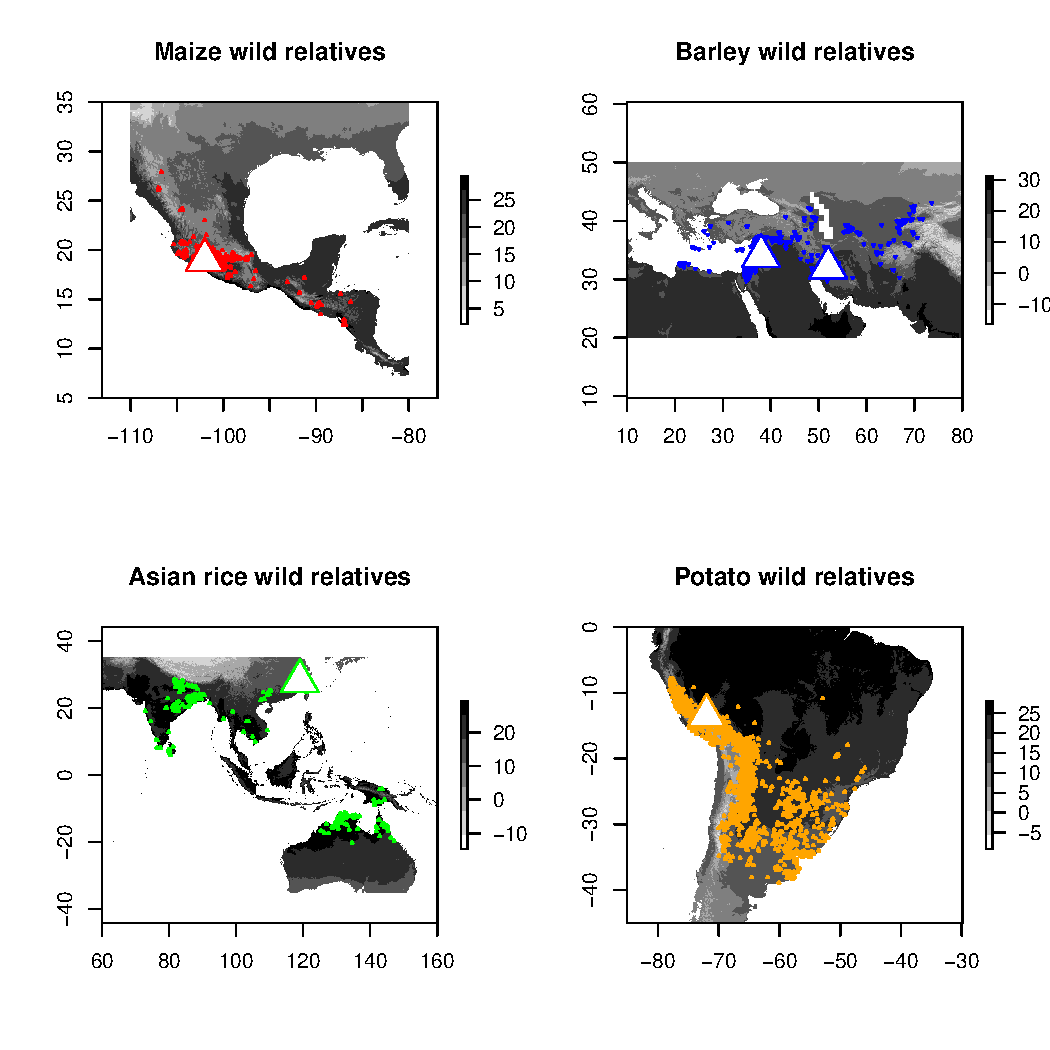
\includegraphics[width=15cm]{temperature_plot_degC.pdf}
	\caption{Map of the natural ranges of wild relatives of four domesticated crops overlayed on average annual temperature. Approximate domestication center for each crop is denoted by a triangle}
	\label{fig:map}
\end{figure}


\begin{enumerate}
\item{Maize:}

The relationship between maize (\emph{Zea mays} ssp. \emph{mays}) and the teosinte \emph{Zea mays} ssp. \emph{mexicana} (hereafter, \emph{mexicana}) offers a prime example of adaptive wild-to-crop introgression.
Maize was domesticated from \emph{Zea mays} ssp. \emph{parviglumis} (hereafter, \emph{parviglumis})  approximately 9,000 BP in the lowlands of the Balsas River Valley in Mexico \citep{matsuoka2002single}.
From this domestication center, maize spread into the highlands of the Mexican Central Plateau, where it came into sympatry with \emph{mexicana}.
Introgression from \emph{mexicana} to maize has been reported based on both morphological \citep{wilkes1977} and molecular \citep{vanHeerwaarden2011, doebley1987} data.
\citet{Hufford2013} first localized \emph{mexicana} introgression to chromosomal regions and provided evidence that it was likely adaptive.
The authors identified nine genomic regions in several maize populations which consistently showed evidence of \emph{mexicana} introgression based on ancestry deconvolution methods including HAPMIX (\textbf{Figure 2}).
These introgressed segments overlapped with QTL that had previously been shown to control anthocyanin content and leaf macrohairs \citep{lauter2004}, traits known to be adaptive at high elevation.
In a growth chamber experiment, the authors demonstrated that maize populations with \emph{mexicana} introgression had increased height (a proxy for fitness) under highland environmental conditions.
Height differences were not detected under lowland conditions, providing further evidence of local adaptation.


Populations of \emph{mexicana} cannot be found outside the highlands of Mexico, yet maize has colonized and adapted to high elevation in a number of other regions.
\citet{Wang2017} employed the ABBA-BABA and $\hat{f_{d}}$ statistics to evaluate if maize with \emph{mexicana} introgression was transferred to other highland regions or whether highland adaptation was obtained \emph{de novo} outside of Mexico.
Overall, analyses revealed that  \emph{mexicana} introgression was pervasive in maize from Mesoamerican high-elevation regions (the highlands of Mexico, Guatemala, and the southwestern United States), but that more distant high-elevation regions (\emph{e.g.,} the Andes) showed no \emph{mexicana} ancestry.
These findings are consistent with previous work suggesting high elevation adaptation in Andean maize likely occurred \emph{de novo} \citep{Takuno2015}.


\begin{figure}[h]
	\centering
	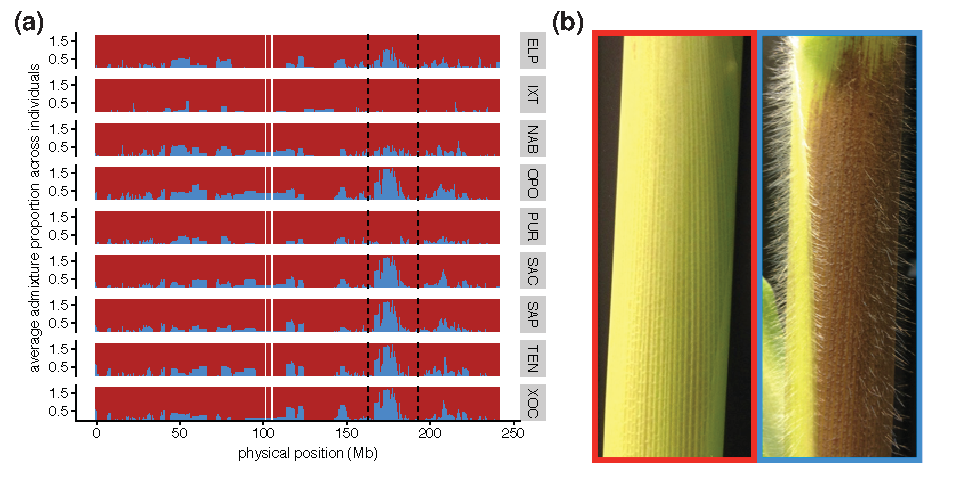
\includegraphics[width=12cm]{./FigsAndTables/Figure1new2}
	\caption{Evidence of adaptive introgression from \emph{mexicana} to Mexican highland maize on chromosome 4. (a) Stacked bar plots of a HAPMIX introgression scan. For each population and chromosomal position, red indicates maize ancestry and blue indicates \emph{mexicana} ancestry. Data obtained from \citet{Hufford2013}. ELP: EL Porvenir; IXT: Ixtlan ; NAB: Nabogame; OPO: Opopeo; PUR: Puruandiro; SAC: Santa Clara; SAP: San Pedro; TEN: Tenango del Aire; XOC: Xochimilco. The dashed vertical lines indicate a previously identified QTL for macrohairs and pigment density in \citet{lauter2004}. (b) Phenotypic differences between maize stems with (blue) and without (red) \emph{mexicana} introgression in QTL affecting presence of pigment and macrohairs. \label{fig:introgressionMaize}}.
\end{figure}

\item{Barley:}

Barley (\emph{Hordeum vulgare} ssp. \emph{vulgare}) was likely domesticated multiple times from wild ssp. \emph{spontaneum} roughly 8,000 to 10,000 BP.
There is clear evidence of one domestication center in the Fertile Crescent \citep{badr2000origin, Morrell2007}, and others have supported additional eastern domestication events, potentially from ssp. \emph{spontaneum} east of the Zagros Mountains \citep{Morrell2007} or from ssp. \emph{spontaneum} var. \emph{agriocrithon} in modern-day Tibet \citep{dai2012tibet}.
However, recent research casts doubt on Tibetan domestication and suggests that var. \emph{agriocrithon} is not a wild relative, but rather a hybrid of domesticated landraces \citep{pourkheirandish2018elucidation}.
Presently, the distribution of wild barley stretches from the eastern Mediterranean to west-central Asia, spanning clines in temperature, precipitation, soil type, and altitude \citep{Morrell2007}.
Cultivated barley is found throughout wild barley's distribution \cite{harlan1966distribution} and crop-wild hybrids are fertile and common when these taxa co-occur.

\citet{Poets2015} recently investigated the range-wide contribution of wild barley to landraces, assessing both genome-wide and geographical patterns of introgression.
This study identified several lines of evidence consistent with wild introgression aiding the expansion and adaptation of domesticated barley.
The authors utilized ancestry deconvolution methods to identify genomic regions of shared ancestry, which linked particular landraces to numerous wild relative populations.
These results suggest landraces may have received wild introgression on a continual basis during post-domestication expansion.
However, barley landraces also showed an excess of ancestry from nearby wild relatives, indicating a prevalence of local and potentially adaptive gene flow.
Limited admixture linkage disequilibrium and small tracts of identity by state suggest substantial recombination has occurred since initial crop-wild hybridization and that even locally introgressed chromosomal regions are ancient, perhaps dating to the early expansion of barley post-domestication.
While these patterns suggest the possibility of adaptive introgression, wild barley haplotypes have yet to be definitively linked to specific adaptations in landraces.

\item{Asian Rice:}

The details of Asian rice (\emph{Oryza sativa}) domestication are still debated.
Certain genetic and archaeobotanical evidence point toward independent domestications of the two prominent varietal groups \emph{japonica} and \emph{indica} from the wild species \emph{Oryza rufipogon} (\emph{rufipogon}, hereafter) in China and the Indian Ganges plain, respectively \citep{fuller2010consilience}, with a potential third domestication event giving rise to the varietal group \emph{aus} in Bangladesh or central India \citep{civavn2015three}.
Other studies support a single domestication in China, with later divergence of \emph{japonica} and \emph{indica} \citep{molina2011molecular, Huang2012} during crop expansion.
For example, \citet{Huang2012} measured genetic distance between a range-wide sample of wild and domesticated rice, finding that \emph{japonica} was likely domesticated near the Pearl River in Guangxi province, China, and that \emph{indica} potentially resulted from hybridization between \emph{japonica} and local \emph{rufipogon} populations in southern and south-eastern Asia.
In a re-examination of these same data, Civ\'{a}\v{n} and colleagues \citeyearpar{civavn2015three} found evidence supporting independent domestications of \emph{japonica}, \emph{indica}, and \emph{aus}, as well as a hybrid origin (\emph{japonica} x \emph{aus}) of aromatic rice.
A recent third analysis by \citet{choi2018multiple} compared these two disparate results and concluded that domestication alleles (including \emph{LABA1}, \emph{PROG1}, and \emph{sh1}) arose during a single domestication event of \emph{japonica}, and were introgressed into several wild \emph{rufipogon} subpopulations (crop-to-wild gene flow), which thereby became the progenitors of other Asian rice varietals.

The findings of \citet{choi2018multiple} bear similarities to a hypothesis posited by Vaughan and colleagues \citeyearpar{vaughan2008evolving} that stresses the potential adaptive significance of crop-wild gene flow in rice.
According to this hypothesis, domestication alleles arose in a single cultivated rice population and subsequently introgressed into diverse cultivated populations (some \emph{japonica}-like, some \emph{indica}-like).
As these domesticated populations spread further into new environments, they potentially received introgression from locally adapted wild relatives, retaining alleles that improved fitness.
While the precise history of domesticated rice remains in question, multiple lines of evidence indicate diverse wild populations have contributed to domesticated germplasm and suggest adaptive introgression may have played a role during the expansion of this important crop.

\item{Potato:}

Modern potato (\emph{Solanum tuberosum}) was likely domesticated approximately 6,000-10,000 BP in southern Peru in sympatry with several wild relatives.
The exact progenitor has remained in question for some time \citep{spooner2005single, pickersgill1977origins, hawkes1988evolution}, but a distance-based phylogeny constructed using genotypic data from a \emph{Solanum} diversity panel recently identified \emph{S. candolleanum} as the most probable progenitor \citep{hardigan2015taxonomy}.
The lack of clarity regarding a progenitor has been due, in part, to extensive post-domestication hybridization between potato and a number of related species.

While potatoes are primarily propagated clonally, farmers do at times promote sexual reproduction for improvement of the crop and development of new cultivars \citep{quiros1992increase}.
Close proximity of domesticated potatoes and wild relatives, active hybridization, and local selection pressure favoring wild haplotypes across a diverse range of biotic and environmental conditions have likely fostered an expansion of genetic diversity within potatoes subsequent to domestication \citep{brush1995potato}.
The prevalence of wild introgression was recently clarified in a broad survey of potato diversity by Hardigan and colleagues \citeyearpar{hardigan2017genome}.
These authors discovered that tetraploid domesticates in particular had received extensive introgression from wild \emph{Solanum}, documenting a continued broadening of the genetic base of potato as it spread away from its Peruvian origin.
In certain cultivars, wild ancestry was estimated at upwards of 30\%.
Genes located within these introgressed regions were more likely to be highly expressed and stress-inducible, and contained loci related to disease resistance, drought tolerance, and heat tolerance, suggesting introgression conferred adaptations critical to survival, possibly facilitating tolerance for new environmental pressures during range expansion \citep{hardigan2017genome}.
\end{enumerate}

These four crop system case studies represent particularly compelling examples of wild and potentially adaptive introgression.
%The four crop systems described in detail here represent particularly compelling examples of wild and potentially adaptive introgression.
However, given their similar histories, many additional crops have likely benefited from wild-to-crop gene flow during post-domestication expansion (\textbf{Table 1}).
Across these four cases studies, some generalities can be observed.
Data thus far indicate that wild introgression is often regional in its extent, but that, in certain cases (\emph{e.g.}, \emph{mexicana} haplotypes detected in maize landraces from the Guatemalan or southwestern U.S. highlands), newly introgressed wild haplotypes can be disseminated more broadly.
Additionally, when functional information is evaluated, as in the maize and potato studies, introgression has been found to occur at loci conferring adaptation to novel conditions not found in a crop's center of origin.
The wild gene flow identified in these case studies raises a number of questions regarding both domestication and adaptation of crops.

\section*{Re-evaluating domestication}

A framework in which crops are domesticated from a single wild population or even a single species is an oversimplification when introgression has been extensive throughout a crop's history.
The addition of ongoing gene flow to our understanding of crop demography could therefore bear on fundamental questions of crop domestication:

\subsection*{Where and from what taxa did a crop originate?}
Depending on the extent of post-domestication gene flow with new wild relatives, identification of a crop's origin may be complicated or confounded entirely.
Introgression between a crop and newly encountered taxa decreases divergence of the crop from these donors.
This signal could be mistaken for origin rather than gene flow.
For example, when determining a single origin of maize from \emph{parviglumis}, Matsuoka and colleagues \citeyearpar{matsuoka2002single} identified a paradox: while \emph{parviglumis} is found exclusively in the lowlands of southwest Mexico, maize with allele frequencies most similar to \emph{parviglumis} was found in the highlands of the Mexican Central Plateau.
Several years later, \citet{vanHeerwaarden2011} resolved the paradox by determining that widespread introgression in the highlands from \emph{mexicana}, which is closely related to \emph{parviglumis}, has caused maize from this region to appear ancestral.
Similarly, as described above, extensive post-domestication adaptive introgression from potato wild relatives long obscured this crop's origin.

Beyond confounding detection of progenitor taxa, extensive introgression may necessitate a more nuanced view of crop origins.
In cases like maize and potato it is important to recognize the substantial contributions of introgressing taxa to modern crops.
While these crops may have originated from a single species or subspecies, the crops as we know them today have a broader genetic base.
Conversely, the domestication histories of barley and rice might best be described as noncentric due to the significant genetic contributions from geographically diverse locations \cite{allaby2015barley}.

\subsection*{When was a crop domesticated?}
Estimates of the timing of initial domestication are often based on levels of sequence divergence between a crop and populations of its presumed progenitor (\emph{e.g.}, \citep{matsuoka2002single, molina2011molecular}).
In highly introgressed domesticates, these estimates will be based on comparison of both crop and introgressant haplotypes to those of the presumed progenitor.
In such cases, divergence time is a mixture of time since domestication and time since split of the progenitor and the introgressing taxa.
This phenomenon, in combination with divergence of modern crop samples from true ancestral crop populations, ongoing evolution of crop progenitors, and genetic structure among wild relative populations, may help explain discrepancies between domestication dates based on genetic and archaeological data.
More accurate estimates of the timing of domestication may be obtained from genetic data by excluding loci that show signatures of introgression or by explicitly including estimates of introgression when modeling a crop's demographic history.

\subsection*{How has genome-wide diversity been shaped by domestication?}

Measurement of the strength of the initial domestication bottleneck may also be impacted by adaptive introgression during the spread of crops.
Crop wild relatives have distinct demographies when compared to domesticates and may therefore have contrasting effective population sizes ($N_e$).
The influence of wild relative introgression on estimates of the domestication bottleneck will depend on a number of factors including the magnitude of gene flow, the $N_e$ of the introgressing taxon, and the strength of selection on haplotypes following introgression.
For example, substantial introgression from a wild taxon with a historically higher $N_e$ will lead to underestimates of the overall strength of the initial domestication bottleneck.

\subsection*{What candidate genes were targeted by selection during domestication?}

Loci targeted by selection during domestication can be identified through so-called ``bottom-up'' approaches based on population genetic signatures \citep{Ross-Ibarra2007}.
Ideally, candidate loci will be identified by first constructing a demographic model representing the history of the domesticate.
In this approach, polymorphism data from neutral loci are fit to potential models of a crop's demography and then statistical tests of selection are used to identify candidate domestication genes under the most likely model.
Due to the uncertainty associated with any given demography, many studies identify domestication loci using a strict outlier approach in which loci showing, for example, the greatest reduction in nucleotide diversity or the highest allele frequency differentiation in the domesticate relative to the wild progenitor are identified as candidates.
Introgression during crop expansion may influence candidate gene detection using both demographic-modeling and strict-outlier approaches.
For example, \emph{mexicana} introgression into maize described above accounts for approximately 20\% of the genome of maize in the highlands of Mexico \citep{vanHeerwaarden2011}.
Takuno and co-authors \citeyearpar{Takuno2015} have shown that a demographic model incorporating this introgression is a significantly better fit to empirical data than a model lacking introgression.
Failure to account for introgression in maize would therefore compromise domestication candidate detection, particularly if a study contained maize samples from the Mexican highlands where \emph{mexicana} introgression is most prevalent.
Likewise, introgression that increased nucleotide diversity in the domesticate or decreased differentiation at domestication loci would confound a strict outlier approach.
However, previous work, also in maize, has shown that known domestication loci are particularly resistant to wild introgression \citep{Hufford2013}, likely due to ongoing selection favoring the domesticated phenotype.
\vspace{5mm}

In summary, since post-domestication gene flow with wild relatives appears frequent during crop histories, investigations seeking to unravel fundamental questions of initial domestication must take this into account in order to accurately estimate parameters of interest.


\section*{Investigating crop adaptation through introgression:}

While research in a subset of crops suggests adaptive wild introgression likely occurred, the scope and dynamics of this process remain poorly described or unexplored in many systems.
In determining the extent and nature of adaptation due to introgression, several questions should be considered:

\subsection*{Do geographic patterns of introgression inform our understanding of adaptation?}
Conservation of the genomic architecture of introgression across individuals,  between populations, and across landscapes can help illuminate whether introgression is adaptive.
For example, if an introgressed chromosomal region is conserved across a broad ecogeographic region, this suggests it may impart adaptation to more widespread environmental or climatic variables (\emph{e.g.}, cool temperatures at high elevation).
On the other hand, if genetic architectures of introgression are conserved across individuals within a population but not across populations in the region, this suggests more local selective pressures (\emph{e.g.}, locally prevalent biotic pressures).
Highly variable introgression across individuals would be more consistent with random gene flow than adaptation.

\subsection*{Over what timescales and in what genomic regions can we reliably detect adaptive introgression?}
Introgressed haplotypes are most easily detected with limited recombination post-hybridization.
Therefore, recent introgressions (limited meioses) or those occurring in low recombination regions such as centromeres or inversions are preferentially detected.
While this can be problematic for the detection of ancient introgression, the fact that recombination degrades tracts of introgression at a relatively constant and predictable rate allows use of the genome-wide distribution of introgression tract lengths to date initial hybridization (as in \citealt{Poets2015}).
Detection of introgression will also be affected by mutation rate, effective population size, the strength of selection on introgressed alleles, and the extent of divergence between donor taxa and a crop's wild progenitor (\emph{e.g.}, highly divergent introgressed haplotypes will be easier to identify).

\subsection*{From which wild taxa will introgression occur?}
As species become substantially diverged gene flow is limited due to Dobzhansky-Muller incompatibilities and other pre- and post-zygotic barriers.
Divergence time may therefore be a useful predictor of the possibility of gene flow between taxa.
Hybridization may also be limited between a crop and a particular wild relative due to genetic load. 
For instance, gene flow from a wild relative with a small long-term effective population size, and correspondingly high genetic load may not be favored by selection.
This effect has been observed in the case of Neanderthal introgression into humans, which was likely limited and relegated primarily to non-genic regions due to the high genetic load found within Neanderthal donor individuals \citep{harris2016genetic}.

\subsection*{Can adaptive introgression inform crop improvement?}

Additional study of introgression in agroecosystems could lead to advances in crop improvement.
As described above, loci underlying the domesticated phenotype can be more clearly identified by removing the confounding population genetic signals of introgression.
Furthermore, adaptive introgression that is demonstrably tied to a specific environment represents a promising source of beneficial alleles that can be directly utilized in breeding to adapt crops to similar conditions.
Finally, as the historic role of wild relatives in the adaptation of crops is clarified, their conservation may be more prioritized, particularly as a resource for breeding in the face of future climate volatility and change.

\section*{Conclusions}

Recent innovations in both high-density marker data and methods for characterizing genome-wide patterns of introgression have helped reveal the extent and timing of gene flow in a number of species.
Application of these data and techniques has led to mounting evidence of crop-wild gene flow following initial domestication in several species.
Substantial post-domestication gene flow with wild relatives can affect inferences regarding domestication and may be an important mechanism through which crops adapted to novel conditions during global expansion.
An accurate understanding of the extent of gene flow is therefore important to both the basic study of crop evolution and to the identification of adaptive alleles for continued crop improvement.
While some studies in crop systems have identified wild introgression, even fewer have effectively linked introgressed alleles to adaptation.
More comprehensive functional analyses and field evaluation will be critical for understanding the evolutionary and adaptive significance of introgression in crops.

\section*{Acknowledgements}
The authors thank Daniel Gates, Peter Morrell, Jeffrey Ross-Ibarra and Jonathan Wendel for comments on a previous version of this manuscript. This work was supported by funding from the National Science Foundation Plant Genome Research Program (IOS-1546719).


\bibliography{bib_gj.bib}

\nolinenumbers

\begin{table}[h]
\small
\rowcolors{2}{white}{gray!25}
\begin{center}
\caption{List of recently developed methods for detecting introgression and examples of their use in empirical studies.} \label{tab:tools}
\begin{tabular}{G{2.8cm}G{3.5cm}G{4cm}G{4cm}}
\\\toprule  
\rowcolor{white}
{\bf Methods}	& {\bf Data Type } &	{\bf References} &  {\bf Applications } \\ \midrule

\rowcolor{gray!25}
{\emph{\bf Divergence}} &   &   &   \\
\rowcolor{gray!25}
Gmin &	biallelic SNP	&  \cite{geneva2015}	 &  \cite{kingan2015}\\
\rowcolor{gray!25}
RNDmin	& phased haplotype	& \cite{rosenzweig2016} &  \cite{roda2017} \\
\rowcolor{gray!25}
$U_{A,B,C(w,x,y)}$ and $Q95_{A,B,C(w,y)}$ & biallelic SNP & \cite{Racimo2015} & \cite{sams2016} \\

\rowcolor{white}
{\emph{\bf Ancestry Deconvolution}} &   &   &   \\
\rowcolor{white}
Hapmix	& phased haplotype; reference panel		& \cite{Price2009}	&  \cite{Hufford2013} \\ 
\rowcolor{white}
RASPberry &	phased haplotype &	\cite{wegmann2011}	 & \cite{christe2016} \\
\rowcolor{white}
MultiMix & phased/unphased genotype; reference panel &	\cite{churchhouse2013} &	\cite{eyheramendy2015} \\
\rowcolor{white}
PCAdmix	 & phased haplotype	 & \cite{brisbin2012pcadmix}	 &  \cite{moreno2014genetics} \\
\rowcolor{white}
LAMP  &	phased haplotypes; reference panel	 & \cite{sankararaman2008}	 & \cite{patterson2012} \\

\rowcolor{gray!25}
{\emph{\bf Phylogenetic Relationship}} &   &   &   \\
\rowcolor{gray!25}
ABBA-BABA/D-statistics	 & biallelic SNP  &	\cite{durand2011}	 &  \cite{heliconius2012} \\
\rowcolor{gray!25}
fd statistic &	biallelic SNP &	\cite{martin2015}  &	\cite{zhang2016genome} \\ 
\rowcolor{gray!25}
five taxon D statistics	& biallelic SNP	&  \cite{pease2015}	& \cite{fontaine2015} \\

\end{tabular}
\end{center}
\end{table} 

\hspace*{-1.5cm}
\begin{sidewaystable}
\caption{\small Extent of evidence for adaptive introgression for major crops including whether hybrids are observed, introgression is detected, and introgression has been shown to be adaptive.} \label{tab:intro}
        \small
    \begin{tabular}{G{4.5cm}G{5.5cm}C{1.75cm}C{2.5cm}C{2.25cm}G{3.5cm}}
        \rowcolor{white}
    \\\toprule  
    {\bf Domesticated Crop}	& {\bf Compatible Wild Relatives} &	{\bf Hybrids} &  {\bf Evidence of Introgression } &	{\bf Evidence of Adaptation} & {\bf Sources}\\ \midrule
    \rowcolor{gray!25}
Apple (\emph{Malus domesticus}) & \emph{M. sylvestris}, \emph{M. orientalis}, \emph{M. baccata}, \emph{M. sieversii}  & X & X & & \cite{ma2017reduced} \\
\rowcolor{white}
Asian Rice (\emph{Oryza sativa}) & \emph{O. rufipogon} & X & X & X & \cite{Huang2012} \\ 
\rowcolor{gray!25}
Barley (\emph{Hordeum vulgare}) & \emph{H. v.} subsp. \emph{spontaneum} & X & X & X & \cite{Poets2015} \\
\rowcolor{white}
Cassava (\emph{Manihot esculenta}) & \emph{M. glaziovii} & X & X & X & \cite{bredeson2016sequencing} \\
\rowcolor{gray!25}
Common Bean (\emph{Phaseolus vulgaris}) & \emph{P. v.} var. \emph{aborigineus, P. v.} var. \emph{mexicanus} & X & X &  & \cite{rendon2017genomic} \\
\rowcolor{white}
Grapes (\emph{Vitis vinifera} subsp. \emph{vinifera}) & \emph{V. v.} subsp. \emph{sylvestris} & X & X &  &  \cite{myles2011genetic} \\
\rowcolor{gray!25}
Maize (\emph{Zea mays} subsp. \emph{mays}) & \emph{Z. m.} subsp. \emph{mexicana}, \emph{Z. m. } subsp. \emph{parviglumis} & X & X & X & \cite{Hufford2013} \\
\rowcolor{white}
Olive (\emph{Olea europaea} ssp. \emph{europaea} var. \emph{sativa}) & \emph{O. e.} ssp. \emph{europaea} var. \emph{sylvestris} & X & X & & \cite{diez2015olive} \\ 
\rowcolor{gray!25}

Potato (\emph{Solanum tuberosum}) & many & X & X & X & \cite{hardigan2017genome}\\
\rowcolor{white}
Soybeans (\emph{Glycine max}) & \emph{G. soja} & X & X &  & \cite{han2016domestication} \\ 
 
\rowcolor{gray!25}
Sorghum (\emph{Sorghum bicolor} subsp. \emph{bicolor}) & \emph{S. b.} subsp. \emph{arundinaceum, S. b.} subsp. {drummondii} & X & X &  & \cite{aldrich1992patterns} \\
\rowcolor{white}

Sunflower (\emph{Helianthus annuus}) & \emph{H. argophyllus}, \emph{H. bolanderi}, \emph{H. debilis}, \emph{H. petiolaris} & X &   &   & \cite{rieseberg2007hybridization}\\
\rowcolor{gray!25}
Tomato (\emph{Solanum lycopersicum}) & \emph{S. pimpinellifolium} & X & X & X & \cite{rick1958role} \\

\rowcolor{white}
 Wheat (\emph{Tritium monococcum, T. dicoccum, T. aestivum}) & \emph{T. m. boeoticum, T. dioccoides, T. urartu, Aegilops speltoides, A. tauschii} & X & X &  & \cite{dvorak2006molecular} \\

    \end{tabular}
\end{sidewaystable}

\end{document}
